\documentclass[conference]{IEEEtran}
\usepackage{graphicx}

\title{DecentraliDrone: A Decentralized, Fully Autonomous Drone Delivery System for Reliable, Efficient Transport of Goods}
\author{
\IEEEauthorblockN{Abdul Aziz A.B}
\IEEEauthorblockA{abdulaziz.ahamed2020@vitstudent.ac.in}
\IEEEauthorblockT{VIT University}

\and

\IEEEauthorblockN{Dhairya Gupta}
\IEEEauthorblockA{dhairya.g2020@vitstudent.ac.in}
\IEEEauthorblockT{VIT University}

\and

\IEEEauthorblockN{Samik Saraswat}
\IEEEauthorblockA{samik.saraswat2020@vitstudent.ac.in}
\IEEEauthorblockT{VIT University}
}
\date{January 1, 2023}

\begin{document}

\maketitle

\begin{abstract}
As the world becomes more interconnected and globalized, the demand for efficient and reliable delivery systems is on the rise. To meet this demand, we propose DecentraliDrone, an innovative drone delivery system that utilizes advanced technology to transport goods autonomously and efficiently. Our system is fully decentralized, meaning that it operates without the need for human intervention and relies on a distributed network of drones and devices to function. One of the key features of DecentraliDrone is its autonomy. The system operates without the need for human intervention, enabling it to operate 24/7 and reducing the risk of accidents caused by human error. Additionally, our system is highly scalable, allowing it to adapt to changing demands and expand its delivery capabilities.
There are several challenges that must be addressed in order to fully realize the potential of DecentraliDrone. These include developing robust communication protocols, ensuring the safety and security of the system, and addressing regulatory and legal issues related to autonomous delivery systems.
The potential applications of DecentraliDrone are numerous and varied, ranging from delivering medical supplies to remote areas to transporting goods between urban centers. By enabling fast, reliable, and autonomous delivery, DecentraliDrone has the potential to revolutionize the way we transport goods and bring us closer to a more interconnected and efficient world.

\end{abstract}\\

\begin{IEEEkeywords}
Reinforcement Learning, OpenCV, Unreal Engine, Swarm, MetaShape, V-SLAM, Autonomous System, Decentralization
\end{IEEEkeywords}

\section{Introduction}
Drone delivery systems have the potential to revolutionize the way we transport goods, offering faster and more efficient delivery options compared to traditional methods. However, most existing drone delivery systems rely on human operators to control the drones and make deliveries, which can limit their efficiency and reliability.

To address these challenges, we propose DecentraliDrone, a fully autonomous and decentralized drone delivery system that utilizes advanced technology to ensure reliable and efficient transport of goods. Our system utilizes a network of drones and devices that are able to communicate and coordinate with each other to ensure timely and accurate delivery.

One of the main advantages of DecentraliDrone is its efficiency. By eliminating the need for human operators, our system can make deliveries faster and more accurately than traditional methods. The autonomous drones are equipped with advanced sensors and navigation systems that enable them to navigate their environment and avoid obstacles, ensuring that deliveries are made safely and timely.

In addition to being efficient, DecentraliDrone is also highly reliable. The decentralized nature of our system means that it is able to operate even if individual drones or devices fail. This ensures that deliveries are not disrupted by technical issues and can continue to be made even in the event of a problem.

One of the key challenges in the development of decentralized autonomous drone delivery systems is ensuring the safety of the drones. To address this, DecentraliDrone utilizes a combination of advanced sensors and algorithms to enable the drones to detect and avoid potential collisions. The drones are also equipped with backup systems to ensure that they can continue to operate even if one system fails.

Another challenge in the development of decentralized autonomous drone delivery systems is integrating them into existing logistics and delivery systems. DecentraliDrone addresses this challenge by utilizing a package management module that tracks the location and status of each package and ensures that they are delivered to the correct destination. The system also utilizes a routing module that calculates the most efficient routes for the drones to take in real-time, ensuring that deliveries are made as efficiently as possible.

There are also potential regulatory and environmental challenges to be considered in the development of decentralized autonomous drone delivery systems. DecentraliDrone addresses these issues by following all relevant regulations and utilizing energy-efficient drones and devices that minimize their environmental impact.

In conclusion, DecentraliDrone is a revolutionary drone delivery system that utilizes advanced technology to transport goods efficiently and reliably. The fully autonomous and decentralized nature of the system ensures that it is able to operate without the need for human intervention and can continue to make deliveries even in the event of technical issues. By addressing the key challenges of ensuring the safety and reliability of the drones, integrating them into existing logistics and delivery systems, and addressing potential regulatory and environmental issues DecentraliDrone is well-positioned to revolutionize the way we transport goods. In the future, we envision a world where DecentraliDrone is widely used for a variety of delivery applications, including same-day delivery of packages and groceries, transportation of medical supplies and equipment, and emergency response deliveries.

Furthermore, the decentralized nature of DecentraliDrone allows it to operate in a wide range of environments, including urban, rural, and remote areas. This makes it a versatile delivery solution that can meet the needs of a wide range of users.

In addition to its practical applications, DecentraliDrone has the potential to have a positive impact on society. By reducing the need for human operators and traditional delivery methods, DecentraliDrone can help to reduce traffic congestion, air pollution, and other environmental issues associated with transportation.

Overall, DecentraliDrone is a promising technology that has the potential to revolutionize the way we transport goods and make a positive impact on society. We look forward to continuing to develop and improve upon this technology in the future.

\section{Related Works}

The research on SLAM has predominantly focused on centralized multi-robot systems, which produce precise maps but suffer from limited scalability, adaptability to unforeseen changes in the environment, and vulnerability to failure in hostile settings. Swarm SLAM techniques have emerged as potential solutions to address these issues by enabling the creation of decentralized, scalable, adaptable, and fault-tolerant maps. However, the adoption of swarm SLAM faces significant technological and financial challenges. It is argued that swarm SLAM could be particularly valuable in scenarios with time or cost constraints, as well as in monitoring dynamic environments. The paper discusses potential applications of swarm SLAM and the primary obstacles that need to be overcome. Nonetheless, the successful implementation of swarm SLAM depends on the availability of suitable, distributed data exchange strategies.\cite{li2018review}.




In both research and education, there is an increasing emphasis on v-SLAM and UAV navigation. However, due to safety restrictions, battery limitations, and the complexity of hardware setups, conducting rigorous physical testing can be time-consuming and costly. To address this issue, a customized simulator has been developed that integrates various localization, mapping, and path-planning modules into a single platform. The simulator features an extended Kalman Filter-based state estimator and a motion control module that runs on the PX4 stack, offering click-and-fly autonomy for UAV navigation. While the simulator has proven to be an effective tool for the development of navigation algorithms and autonomous systems, it cannot replicate the simulation in real-life drones due to the complex hardware setup, safety precautions, and battery constraints that would necessitate extensive physical testing.\cite{zhou2018routing}.




The article presents a survey of SLAM and data fusion techniques and critically evaluates current SLAM implementations in robotics and autonomous vehicles, assessing their applicability and scalability to UAVs. The research bridges the gap between SLAM and data fusion in UAVs while also comprehensively surveying related object detection techniques, such as visual odometry and aerial photogrammetry. The paper begins with an introduction to applications where UAV localization is required, followed by a discussion of multimodal sensor data fusion analysis mounted on UAVs. Various SLAM techniques, such as Kalman filters and extended Kalman filters, which are used for scene perception, mapping, and localization in UAVs, are also explored.\cite{wang2018survey}.

The study aims to reduce the impact of errors caused by different sensor resolutions by employing data fusion techniques. The authors suggest that the data fusion process could benefit from machine learning techniques to make it more end-to-end, while Bayesian SLAM could be made more intelligent with the use of deep learning techniques. However, the authors also acknowledge the challenges associated with data fusion, such as uncertain and imprecise data, processing interfaces, noise, and reliability issues.issues\cite{kegeleirs2021swarm}.




The authors propose a novel estimator for simultaneous localization and mapping system to be applied to UAVs, relying on an Extended Kalman Filter. Data fusion is also utilized by combining data from an orientation sensor (AHRS), a position sensor (GPS), and a monocular camera as parameters to the Kalman estimator. The inclusion of camera measurements into the system considerably improves the estimation of the trajectory of the vehicle, compared with using only the measurements from the position sensor. The suggested method is similar to monocular SLAM systems, but a multi-sensor approach is used to address technical issues. The use of a stochastic triangulation methodology to estimate feature depth helps to overcome the problem of metric scale recovery.

The visual data is obtained with an integrated camera in the flying vehicle pointing to the ground.The suggested method is similar to monocular SLAM systems, which employ a single camera to simultaneously estimate a map of visual features and the trajectory of the camera. To get over some of the technical issues with monocular SLAM systems, a multi-sensor approach is used to make use of the collection of sensors that are frequently found in UAVs. The suggested method relies on a stochastic triangulation methodology to estimate feature depth. The fact that the metric scale of the environment can only be recovered with a known factor if no extra information is added into the system presents another significant problem when using monocular vision\cite{chen2022end}.




The paper also describes a SLAM system designed for low-cost commercial aerial platforms with limited onboard computing capacity. The system uses a minimum onboard sensory configuration of a monocular camera, an Inertial Measurement Unit (IMU), and an altimeter to calculate the pose and environment map of the platform. The authors have also addressed the challenge of GPS-denied or GPS-weak environments in this SLAM system. The system uses an Extended Kalman Filter to estimate the platform’s pose and the environment map, which integrates information from the monocular camera, IMU, and altimeter. The use of low-cost sensors is intentional in this SLAM system, as it is designed for low-cost commercial aerial platforms. Using more sophisticated sensors would increase the cost of the system, which would defeat the purpose of developing a low-cost SLAM system.


The system uses an Extended Kalman Filter to estimate the platform's pose and the environment map. This filter integrates information from the monocular camera, IMU, and altimeter to estimate the position, orientation, and velocity of the platform, as well as the environment map. The use of an altimeter, in addition to the camera and IMU, helps to improve the accuracy of the estimated altitude, which is crucial for accurate mapping.

It is worth noting that the use of low-cost sensors is intentional in this SLAM system, as it is designed for low-cost commercial aerial platforms. Using more sophisticated sensors would increase the cost of the system, which would defeat the purpose of developing a low-cost SLAM system. Therefore, while using an orientation sensor would improve the system's accuracy, it would also increase the system's cost\cite{gupta2022slam}.



The paper provides a detailed, experiment driven comparison between decentralized and centralized behaviour in Unmanned Autonomous Vehicles. The authors place the existing claims such as decentralized control in drones performing better in environments with randomized obstacles on the table and investigate these via experimental findings.

They manage to prove that more decentralized control will provide better scalability and disprove the superiority in performance of decentralized drones under randomized obstacles.

The researchers could have increased the generality of the comparisons made by averaging over several other possible tasks rather than being ad hoc comparisons for specific ones\cite{mahdoui2019multiUAV}.




This paper proposes a multi-UAV framework for SLAM-based cooperative exploration under limited communication bandwidth. It uses a RGB-D based grid mapping and group leader decision making with a new utility function that takes into account each robot distance in the group from the unexplored set of targets, allows to simultaneously explore the environment and to get a detailed grid map of specific areas in an optimized manner.

The paper also makes improvements in memory consumption by reducing the shared data volume by exchanging only the frontier points of the computed local grid map. It also presents substantiative gains in average exploration time and distance travelled.

A big shortcoming of the paper though, is the absence of any obstacles in the environment. This is due to the concave shape assumption of the local maps. Important to note here that out project emulates an environment filled with obstacles of several kinds\cite{munguía2016vslam}.




In this paper, researchers propose a decentralized and distributed collaborative SLAM algorithm called  SLAM. This algorithm has high local accuracy and global consistency, and the distributed architecture allows it to scale up.  SLAM covers swarm state estimation in two scenarios: near-field state estimation for high real-time accuracy at close range and far-field state estimation for globally consistent trajectories estimation at the long-range between UAVs.

This method capable of being applied in various scenarios is robust to transient loss of communication and network delays. Experimental results reveal real-time high-precision local localization capability and real-time high-precision relative localization when the UAVs are near each other.

There are quite a few limitations for this paper which include limited swarm scale growth due to communication and front-end computing capabilities. Relative measurements including UWB and visual recognition are not introduced due to SLAM being a more traditional v-SLAM work\cite{lópez2017sensorial}.




This study presents an unique hybrid multirotor drone architecture that stabilises the drone using four electric motors in addition to two petrol engines, which supply the majority of the lift force.

The main advantage of using this propulsion system is that it is aimed at optimising and exploiting their respective pros, such as reduction of the total energy consumption rate and increase in the time of flight. Taking inspiration from this hybrid system we would be incorporating it into our system. A hybrid gas-electric multirotor drone can already fly longer than a fully electric drone, according to simulation and experiment results.

One of the limitations regarding this would include the minor gasoline emissions in the environment. The simulation and the experimental results specified the optimal gas-to-electric thrust ratio, the fuel amount, and the battery capacity in which all the energy reserves were depleted simultaneously. This ratio can differ from one design to another based on the fuel tank size, battery capacity used, motors and engine types, and drone weight\cite{stolaroff2018energy}.




In this paper, a detailed study highlighting the use of automated, unmanned aerial vehicles(drones) to deliver commercial packages and the significantly shifting energy use in the freight sector was done.The study's goal is to demonstrate that drones use less energy per package-kilometer than delivery trucks, accounting for the additional energy needed for the warehouse as well as the greater distances travelled by drones per package greatly increases the life-cycle impact. Shedding light on careful deployment of these drones, would result in significant reduction of greenhouse gas emissions and energy use in the freight sector when it comes to drone-based delivery systems.

The main advantage of drone based delivery system in contrast to conventional ground vehicle delivery systems comes down to the point that batteries and fuel cells in drones are higher energy efficiency than combustion, lower noise, next to none air emissions at the point of use and possible reduced greenhouse gas impacts via low-carbon electricity storage in batteries or hydrogen produced via low-carbon methods.

Limitations of this include the implementation of the entire system and the gradual change from the conventional delivery system to drone-based delivery systems\cite{jarrah2022flight}.



Loop closure is an essential concept in SLAM systems. It’s the process of detecting a previously visited location in a new observation, which enables the system to correct its map and estimate the robot's position. This process helps to reduce mapping and localization errors and improves the overall accuracy of the system. Loop closure is a crucial step in maintaining consistent maps over long periods and can increase the robustness and reliability of SLAM systems.

Deep neural networks have been applied to various tasks related to loop closure, such as feature extraction, place recognition, and relocalization enabling more accurate and reliable mapping and localization.

The methods include Visual-Based Loop Closure Detection and Lidar Based Loop closure detection and Deep learning-augmented segment-based loop detection method. 

LIDAR sensors fails in changing environment and weather conditions, where vision based loop closure methods are sensitive to illuminations. There is a need of hybrid method which can combine both vision as well as LIDAR for a perfect combination\cite{arshad2021loop}.


In the development of large-scale systems, effective cost reduction and flexibility enhancement provide a major path planning and work allocation issue. One of the main technologies for attaining autonomous driving of UAVs is coverage path planning. However, due to its NP-Hard computational complexity, it is challenging to find the best solutions. The coverage path planning issue for autonomous heterogeneous UAVs on a finite number of regions is examined in this research. 

In order to exhaustively search the solution space and generate the best flight paths for autonomous UAVs, an accurate formulation based on mixed integer linear programming using models of separated regions and heterogeneous UAVs is used. 

Then, drawing inspiration from density-based clustering techniques, we develop a novel clustering-based algorithm to group regions into clusters and determine roughly ideal point-to-point UAV flight paths so that coverage tasks can be completed accurately and effectively\cite{chen2022coverage}. 




There has been progress in developing safe path planning for obstacle avoidance in autonomous vehicles.

The technique combines path pruning, smoothing, and optimization with geometric collision detection to increase planning effectiveness. It is based on the RRT algorithm. Route pruning, a necessary step before path smoothing, is done to eliminate the duplicate points produced by the random trees so that a new path can be created that avoids running into the obstacles.

Path smoothing modifies the path to make it continuously differentiable with curvature that the vehicle can apply. A "near"-optimal path with the lowest distance among the possible paths is chosen through optimization to maximize motion efficiency.  Improvements are done to pruning and smoothing & optimization with help of bezier curves

The experiment has been carried out in a static environment where the obstacles are static and not changing but in real-world scenarios, an open-world approach is required and the autonomous bot has to detect obstacles dynamically and non-deterministically\cite{yang2021rrt}.




A robot needs to be able to navigate even in a dynamic environment with potential obstacles and does always not have any prior information about its environment. The only way to make robots able to navigate is to represent the environment in some form. Generating a 3D map online appears to be the starting point for a complete autonomous navigation in a 3D world. hybridized solutions offer improvements in the performance of SLAM, especially with respect to aggressive motion, lack of light, or lack of visual features

Visual sensors had been the main research direction for SLAM solutions because they are inexpensive, capable of collecting a large amount of information, and offer a large measurement range. They are of 2 types: feature based v-SLAM, Direct-SLAM, RGB-D SLAM, Event-Camera SLAM, Visual SLAM.

They explained about Visual-Lidar SLAM, which consists of EFK Hybridized SLAM and improved Visual SLAM. Among all the ways of implementing such a SLAM, the hybridized framework is the least studied. Creating a common SLAM framework using visual information and laser range seems to be a real challenge. A more tightly coupled LiDAR-vision sensor fusion algorithm is not fully investigated in the literature yet and should be studied\cite{debeunne2020vlidar}.




Choosing an appropriate path planning algorithm helps to ensure safe and effective point-to-point navigation, and the optimal algorithm depends on the robot geometry as well as the computing constraints, including static/holonomic and dynamic / non-holonomically constrained systems, and requires a comprehensive understanding of contemporary solutions. The goal of this paper is to help novice practitioners gain an awareness of the classes of path planning algorithms used today and to understand their potential use cases—particularly within automated or unmanned systems.

Possible Algorithms: Dijkstra (normal, improved, multi-layed, Floyd), A* algorithm (hierarchical, improved, Hybrid, Guided Hybrid, with smart heuristics, lifelong, with equal step sampling, diagnoal), Dynamic A* (D*) (normal, lite, enhanced, field), RRT* (connect, sensor based, RRT*), Genetic algorithms, Ant Colony Algorithms, slime mold based optimization, Improved ant colony optimization, Adaptive ant colony, Enhanced Ant Colony Algorithm, Bidirectional ant colony and firefly algorithms\cite{karur2021path}.




Swarm intelligence has received much research attention in recent years. As a typical application of swarm intelligence, swarm of drones systems generally exhibit decentralized control achieved through simple agent behaviors and interactions developing a self-organization that is considered an emergence of order from the system. 

Much of the work conducted in the Mobile Ad Hoc Networks (MANETs) and Vehicular Ad Hoc Networks (VANETs) field does not approach the unique features of the swarm networks. Swarm networks may change from slow dynamic to dynamic; have intermittent connections and fluid configuration. While it is thought that ad hoc mesh network would be most appropriate for swarm networks. Such networks are low cost cooperative solution for wireless connectivity. While routing, it should have self healing capabilities in case nodes breakdown.

Instead of routing, a flood technique can be used as it is simplistic and reliable but can use more power even when such a resource is limited as well as avoiding ‘broadcast storms’. 

Factors such as energy consumption, range and latency should be taken into consideration when using the ad hoc communication strategies\cite{cui2017brief}.




Swarm intelligence (SI) is concerned with the collective behaviour that emerges from decentralised self-organising systems, whilst swarm robotics (SR) is an approach to the self-coordination of large numbers of simple robots which emerged as the application of SI to multi-robot systems. 

An efficient physics- based model of fire propagation and a self-organisation algorithm for swarms of firefighting drones are developed and coupled, with the collaborative behaviour based on a particle swarm algorithm adapted to individuals operating within physical dynamic environments of high severity and frequency of change.

They use Particle Swarm Algorithms (PSO’s) to achieve these tasks, taking into considerations: the trajectory difference equation, neighbourhood structure, dynamic structure of the mesh, etc\cite{innocente2019self}.




This paper introduces a novel dynamic optimization problem applied to Unmanned Aerial Vehicle (UAV) search and rescue scenarios, named the Moving Peak Drone Search Problem (MPDSP). It utilizes the dynamic environment generator of the well-known Moving Peak Benchmark (MPB) and it is formulated as a maximization problem, with additional constraints imposed by the use of UAVs. 


Coverage based Path planning algorithms proposed which can be further classified into memory based, prediction method based, self-adaptive methods and multi-population methods. Doing dynamic optimization using a fleet of UAVs for searching a  large area is desired\cite{kyriakakis2021moving}.


\section{Proposed Methodology}

\graphicspath{ {./images/} }
\includegraphics[width=8.5cm, height=5.75cm]{td3_algo.png}\\
\caption{Figure 3.1: Proposed Methodology Network}\\\\
\\\
\graphicspath{ {./images/} }

\includegraphics[width=8cm, height=2.5cm]{td3_math_eqns.png}\\\\

Time and Space Complexity Associated with TD3-
The time and space complexity of the TD3 algorithm depend on several factors such as the size of the state and action spaces, the number of layers and neurons in the neural networks, the batch size used for updates, and the length of the training process. 
Overall, the time and space complexity of the TD3 algorithm depend heavily on the size of the neural networks and the batch size used for updates. As these can be adjusted based on the available computational resources, it is difficult to give a general estimate of the complexity of the algorithm. However, it is safe to say that TD3 can be computationally expensive to train, especially for large state and action spaces.


\subsection{Basic Architecture Flowchart}\\

\graphicspath{ {./images/} }
\includegraphics[width=8.5cm, height=8cm]{architecture_new.png}\\
\caption{Figure 3.2: Architecture Flowchart}\\\\
\\
\caption{The customer will raise the request for the purchase and delivery of a specific item through the app interface. The app interface consists of Destination details of the customer, progress updates of the delivery and the payload specifications, i.e., the order details in terms of weight, dimensions and other attributes. The delivery recipient will acquire a unique ArUco marker code mapped to the unique delivery. The recipient has to find a suitable flat surface and place the marker code at the respective position after printing it. Each unique delivery will be mapped to a pair of drones within the drone swarm. The delivery vicinity details will be given as input to the drone unit for the implementation of autonomous delivery. With the help of Path planning algorithms such as TD3 the drone unit will navigate towards the destination vicinity autonomously. These algorithms will ensure the obstacle avoidance, course correction and smooth and effective path planning for reaching the destination. A pair of drone will be assigned to each delivery to ensure smoothness in the delivery as 1 drone will carry the payload and implement V-SLAM while other drone will be giving visual aide and extending the vision of the first drone. This data helps in course correction and precise and accurate navigation to the destination vicinity. Once the drone unit reaches the destination vicinity. After reaching the destination vicinity, the drone unit pair would lower the altitude and start searching for the ArUco marker in the compound using openCV component. If the marker is found and matched by the drone unit, then the drone unit would complete the delivery. After completing the delivery, it would update in the app interface and the logger about the progress and return back to drone dispatch spawn unit. In case the marker is not found or found in an unsuitable environment for completing the delivery, the drone unit would raise a request/alert in the app interface. The recipient will have to respond within a time limit and fix the placement of ArUco, if these conditions are met then the raised request is accepted and the drone unit can proceed with the delivery procedure. If the recipient fails to respond to the request within the specific timeframe, the drone unit would return back to the drone dispatch spawn unit and log that scenario as an incomplete delivery/failure. }


\subsection{Swarm Schematics}\\
\graphicspath{ {./images/} }
\includegraphics[width=8.5cm, height=10cm]{Decentralized_Structure.png}\\
\caption{Figure 3.3: Decentralized Swarm Structure of Drone Network}\\\\
\caption{ This schematic explains the basic workings behind the communications involved among the swarm of drones that are deployed, being a decentralised system, they check in on each other for the delivery states and carry out the delivery screening process where they travel around the delivery point and drop the packages where and when required. The drones also keep track of the individual check ins so that when one of the drones faults to an unfortunate circumstance, the system balances itself by sending in a replacement by peer communication via the group check in feature.
}\\

\subsection{Communication Schematics}\\

\graphicspath{ {./images/} }
\includegraphics[width=8cm, height=12cm]{communication_schematics.png}\\
\caption{Figure 3.4: Drone Activity Diagram}\\\\
\caption{ The following diagram gives a sharp overview of the communication that occurs among the drones to make successful deliveries, being in a decentralised system, the drones are their own controller entity as a whole system, the success of the system is considered as a group effort rather than a singular entity’s success, keeping this in mind, the drones communicate with each other to make sure that the deliveries are made. The communication is done through cellular towers present across the region where the drones are deployed for delivering the goods.
}\\

\subsection{Functional Quad-rotor Schematics}\\

\graphicspath{ {./images/} }
\includegraphics[width=8.5cm, height=6.5cm]{quad-rotor_schematics.png}\\
\caption{Figure 3.5: Single Drone Schematic Diagram}\\\\
\caption{ The following diagram explains the functioning of a singular entity from the system of swarm. Each quad-rotor entity has its own guidance system that is line of sight based, acting upon which the motors and propellers are instructed to take the ascend or descend of the drone, it uses computer vision algorithms to perform obstacle detection and avoidance, the guidance system gives the appropriate trajectory for the drone to take in order to make a successful delivery happen in accordance to the environmental factors that are laid upon in its path. The Guidance system takes the inputs from the navigation system and performs the appropriate logical decisions to map out the path for the drone.
}\\

\subsection{Takeoff and Landing for VTOL Schematics}\\

\graphicspath{ {./images/} }
\includegraphics[width=9.0cm, height=6.5cm]{takeoff_landing.png}\\
\caption{Figure 3.6: Takeoff and Landing pre-flight schematics for single drone}\\\\
\caption{ The following diagram explains the take off and landing sequence of the drone, since the drone is said to land on specific markers per delivery, a system of precision landing is brought into play, this is used to successfully land the drone at the spot and take off after the delivery, the system is an implication of a VTOL based system which uses the appropriate altitude and position control. Fall detection systems are also implemented to alert the others in the swarm for a due maintenance for the drone and the incomplete delivery, which may or may not be taken in charge by the other drones in the vicinity.  
}\\

\subsection{App Schematics}\\

\graphicspath{ {./images/} }
\includegraphics[width=9.5cm, height=7.5cm]{app_schematics.png}\\
\caption{Figure 3.7: Drone Delivery Application Schematics}\\\\
This diagram explains the workings that are underlying in the application that is developed specifically for this system to be achieved, it explains the confirmation of the buyer to whom the goods are delivered and the unique ArUco markers that are generated for each deliveries, the items involved in the delivery, the locations to be delivered and so on.\\

\section{CAD model of the Hybrid drone}\\

\begin{enumerate}
    \item Drone is in the Quad(X) Configuration.\\
    
    \graphicspath{ {./images/} }
    \includegraphics[width=8cm, height=4cm]{X_config.png}\\
    \caption{Figure 4.1: Drone in X Config}\\

    \item This is the orientation showing a hybrid power based drone CAD model. \\

    \graphicspath{ {./images/} }
    \includegraphics[width=8cm, height=4cm]{config2.png}\\
    \caption{Figure 4.2: Hybrid Model}\\

    \item Synthetic Dome covering the brain of the drone (sensitive sensors, flight controller and the microcontroller/microcomputer integrated on top).\\

    \graphicspath{ {./images/} }
    \includegraphics[width=8cm, height=4cm]{dome.png}\\
    \caption{Figure 4.3: Protective Dome of Drone}\\
    
    \item Orientations showing fuel tank as hybrid power source of drone.\\

    \graphicspath{ {./images/} }
    \includegraphics[width=8cm, height=4cm]{fuel_tank.png}\\
    \caption{Figure 4.4: \textit{Side View}}\\\\


    \graphicspath{ {./images/} }
    \includegraphics[width=8cm, height=4cm]{fuel_tank2.png}\\
    \caption{Figure 4.5: \textit{Bottom View}}\\\\

    \item The robotic manipulator based component integrated to handle the associated payload.\\

    \graphicspath{ {./images/} }
    \includegraphics[width=8cm, height=4cm]{manipulator.png}\\
    \caption{Figure 4.6: Drone tentacular manipulators}\\
    
    
\end{enumerate}



\section{Result Comparison of Existing and Proposed System}
\textit{A Brief Overview of Parameters}\\


\textbf{Best Y}\\

The \textit{"best Y vs episode" }graph shows the maximum reward achieved by the agent in each episode during training. The graph is useful for evaluating the overall performance of the agent during training. The graph shows a steady increase in the maximum reward achieved over the course of training, indicating that the agent is improving its performance.\\

In the early episodes of training, the maximum reward achieved may be low but as it progresses, the maximum reward achieved should increase as the agent becomes more skilled at selecting actions that lead to higher rewards.
The shape of the graph can vary depending on the specific environment and hyperparameters used for training. However, in general, it should show a positive trend over time. If the graph shows a plateau or a decline in the maximum reward achieved, it may indicate a problem with the training process or the environment. \\




\textbf{Actor loss}\\

The graph of \textit{“Actor loss vs episodes” } shows how the loss of the actor changing over the course of training. The actor loss is a measure of how well the actor can select actions that lead to higher rewards. Typically, the actor loss decreases over the course of training as the actor becomes better at selecting actions.\\

In the early episodes of training, the actor loss is high as the actor explores the environment and tries out different actions. As training progresses, the actor becomes more confident in its actions, and the loss decreases. If the actor loss does not decrease over the course of training, it indicates a problem with the training process or the environment itself. In such cases, it may be necessary to adjust the hyperparameters or try different training techniques to improve performance.\\

\textbf{Critic loss}\\

\\ The \textit{critic loss vs episode graph} shows the loss of the critic changing over the course of training. The critic loss is a measure of how well the critic can estimate the value of the current state. Critic loss decreases over the course of training as the critic becomes better at estimating the state value. 

In the early episodes of training, the critic loss may be high but as it progresses, the critic becomes more confident in its estimates, and the loss decreases. If the critic loss does not decrease over the course of training, it indicates a problem with the training process or the environment itself. In such cases, it may be necessary to adjust the hyperparameters or try different training techniques to improve performance.\\

\textbf{Level}\\

\\ The \textit{level vs episode graph} shows how the agent's performance on different levels or stages of the environment changes over the course of training. This graph is particularly useful when training the agent on environments with different levels or stages, such as video games with multiple levels. Each point on the graph represents the agent's performance on a particular level or stage during a specific episode of the training process. The performance can be measured by different metrics such as cumulative reward, time taken to complete the level, or accuracy.\\

This graph can provide valuable insights into how the agent is progressing through the levels or stages of the environment. Ideally, the graph should show a steady increase in performance on each level over the course of training. If the agent is struggling on certain levels or stages, this can be identified by a plateau or a decline in performance on the corresponding levels.\\

The shape of the graph can vary depending on the specific environment and hyperparameters used for training. In general, the graph should show a positive trend in performance over time. However, there may be some variability in performance on individual levels or stages, which can be influenced by factors such as the level's difficulty, the randomness of the environment, or the agent's exploration strategy.\\

\textbf{P max}\\

\\ The \textit{"p max vs episode"} graph shows how the maximum probability of the actions selected by the actor changes over the course of training. The maximum probability (p max) is the highest probability assigned by the actor to any action in each state.\\

Ideally, the graph should show a decreasing trend in p max over the course of training, indicating that the actor is becoming more confident in its actions and selecting a wider range of actions.\\

In the early episodes of training, the p max may be high but as it progresses, the actor becomes more confident in its actions, and the p max decreases. This is a desirable outcome as a high p max indicates that the actor is not exploring enough and is potentially stuck in a suboptimal policy.\\
If the p max does not decrease over the course of training, it may indicate a problem with the training process or the environment itself. In such cases, it may be necessary to adjust the hyperparameters or try different training techniques to improve performance.\\

\textbf{Score}\\

\\ A \textit{"score vs episode graph"} is a common way to visualize performance. As the agent learns and improves its policy and value functions through training, one expects to see an upward trend in the score vs episode graph. In the beginning, the agent's performance may be poor, and the score may fluctuate wildly. As the agent learns, however, the score should become more consistent and gradually increase.\\

\textbf{Step}\\

A \textit{"step vs episode graph"} is another way to visualize the performance of a reinforcement learning algorithm. The x-axis represents the episodes or iterations of the algorithm, and the y-axis represents the total number of steps taken by the agent in each episode.\\

Each step represents an interaction between the agent and the environment, where the agent selects an action based on its current policy, receives a reward from the environment, and transitions to a new state. The goal of the agent is to learn a policy that maximizes the cumulative reward over many steps.\\

\textbf{Action}\\

The \textit{"Average action vs episode" graph} shows how the average action taken by the agent changes over time as it interacts with the environment. The average action is typically calculated by taking the mean of the actions taken by the agent across a given episode or time step. It can provide insights into how the agent is exploring the environment and making decisions.\\

If the average action remains constant or fluctuates significantly over time, it may indicate that the agent is not effectively exploring the environment or is having difficulty learning an optimal policy.
On the other hand, if the average action decreases over time, it may indicate that the agent is becoming more conservative in its decision-making and focusing on exploiting known high-reward actions. This behavior may be desirable in certain scenarios, such as when the environment is relatively stable and the agent has learned a good policy.\\

Alternatively, if the average action increases over time, it may indicate that the agent is becoming more exploratory and trying out new actions in the environment. This behavior may be desirable in scenarios where the agent needs to discover new high-reward actions or adapt to changes in the environment.\\

\textbf{Q value}\\

\textit{Q-values} represent the expected reward an agent can receive by taking a specific action in a specific state. The Q-value function is a key component in many RL algorithms, such as Q-Learning and SARSA.\\

The x-axis of the graph represents the number of episodes the agent has completed during its training, while the y-axis represents the average Q-value of the learned policy. Typically, the graph will show a gradual increase in the average Q-value as the agent gains more experience and learns more about the environment. This is because the agent is constantly updating its Q-value estimates based on the rewards it receives from the environment.\\

The shape of the average Q-value versus episodes graph can reveal important information about the learning progress of the agent. For example, a steep increase in the average Q-value in the early episodes may indicate that the agent quickly learns about the environment and finds a good policy. On the other hand, a slower increase in the average Q-value may indicate that the agent is having a harder time learning, and may require more training or a different algorithm.\\

\textbf{Average Velocity}\\

The \textit{average velocity versus episodes graph} is a way of visualizing the learning progress of an RL algorithm in a control task where the goal is to control the velocity of an agent. \\

In this graph, the x-axis represents the number of episodes the agent has completed during its training, while the y-axis represents the average velocity of the agent over those episodes. The graph typically shows a gradual increase in the average velocity as the agent gains more experience and learns more about the environment.\\

In this graph, the x-axis represents the number of episodes the agent has completed during its training, while the y-axis represents the average velocity of the agent over those episodes. The graph typically shows a gradual increase in the average velocity as the agent gains more experience and learns more about the environment.\\


\subsection{Recurrent Advantage Actor Critic Agent for Airsim }\\

\textbf{RA2C}\\
The Advantage Actor-Critic (A2C) algorithm is a reinforcement learning algorithm that combines two approaches: policy gradient and value function estimation. It is commonly used for solving continuous action space environments, where the optimal action cannot be easily determined by the agent. It consists of 2 components: an actor and a critic. The actor is responsible for selecting actions based on the current state, critic evaluates the value of the current state. They work together to improve the agent's performance in the given environment.\\
The actor takes current states as the inputs and outputs a probability distribution over the possible actions. The critic takes the current states as input and outputs an estimate of the state's value. The value function estimate represents expected cumulative reward the agent receives from that state onwards.\\
During training, the agent interacts with the environment to receive rewards and updates the actor and critic. The actor's parameters are updated with the policy gradient method, which encouraging agent to take actions that lead to higher rewards. The critic's parameters are updated using the difference between the estimated value and the actual reward received.\\
The "advantage" in the name refers to the difference between the estimated and the expected value from the current state. This advantage signal is used to update the actor and encourage actions that lead to higher rewards. A2C has several advantages over other reinforcement learning algorithms as it is computationally efficient, and it converges quickly and allows for continuous action spaces, which can be difficult to handle with other methods.\\


\textbf{Best Y}\\

\\
\graphicspath{ {./images/} }
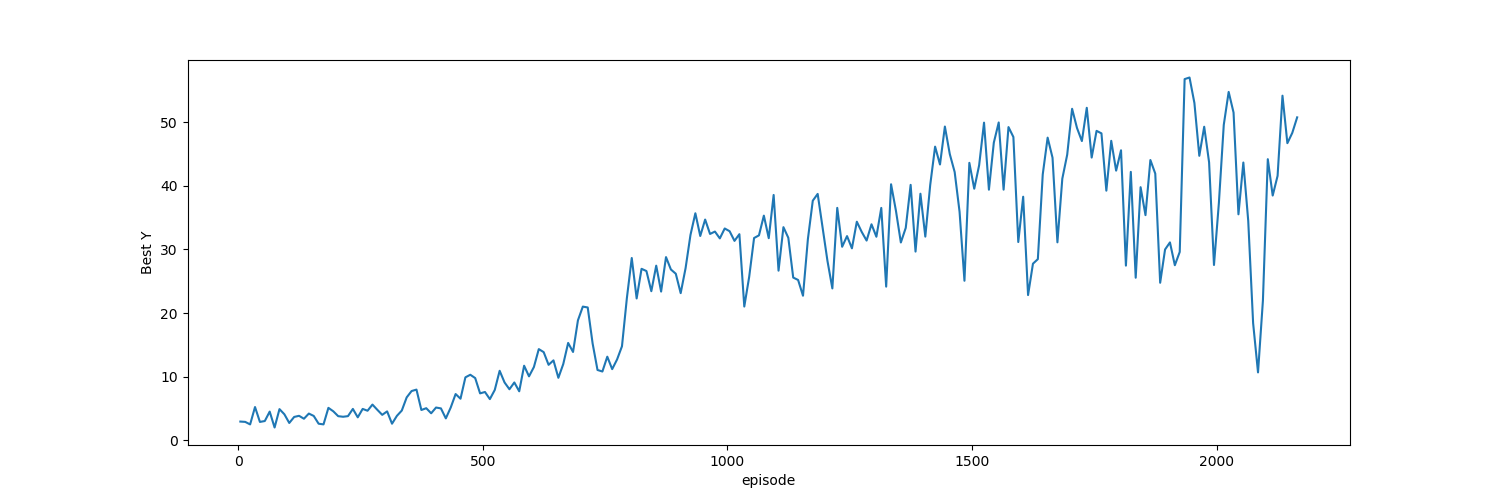
\includegraphics[width=9.5cm, height=4cm]{Best Y.png}
\caption{Figure 5.1: When Best Y graph increases, it typically means that the agent is learning and improving its performance over time. Specifically, it suggests that the agent is finding better policies for interacting with the environment, resulting in higher rewards or better performance.
\\ }\\


\textbf{Actor loss}\\


\graphicspath{ {./images/} }
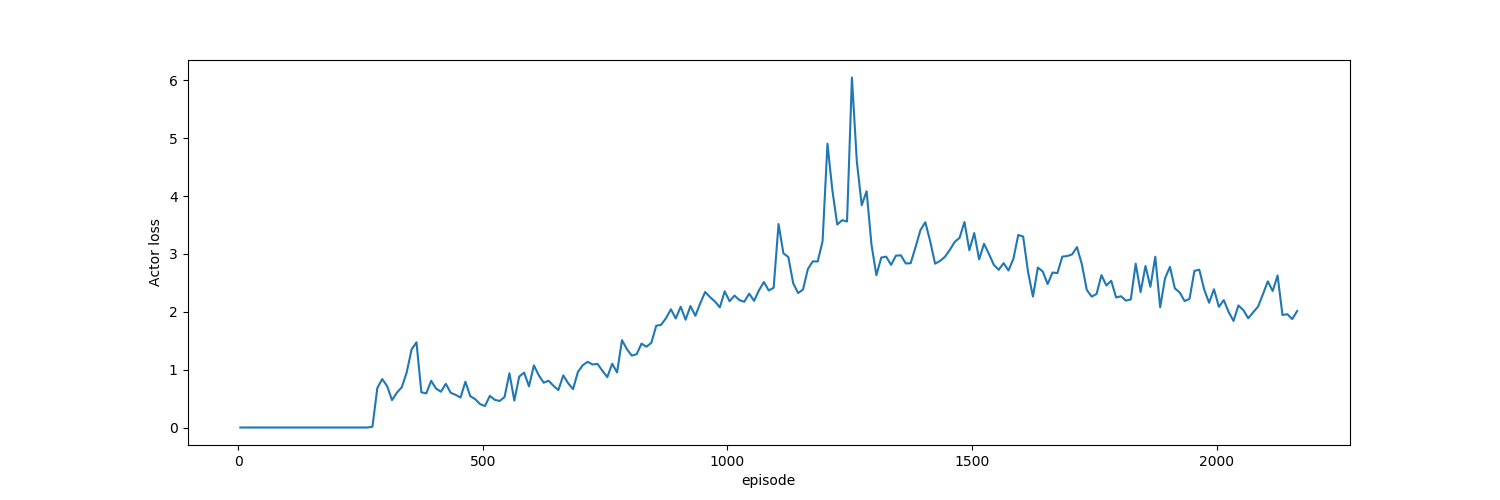
\includegraphics[width=9.5cm, height=4cm]{Actor loss.png}
\caption{Figure 5.2: Actor loss graph remains the same over time, it suggests that the actor network has converged to a local minimum, and is no longer improving its policy. This can happen when the agent has reached a plateau in its learning, and has found a sub-optimal policy that is "good enough" for the current task. In this case, further updates to the actor network may not result in significant improvements in performance.
 }\\

\textbf{Critic loss}\\

\graphicspath{ {./images/} }
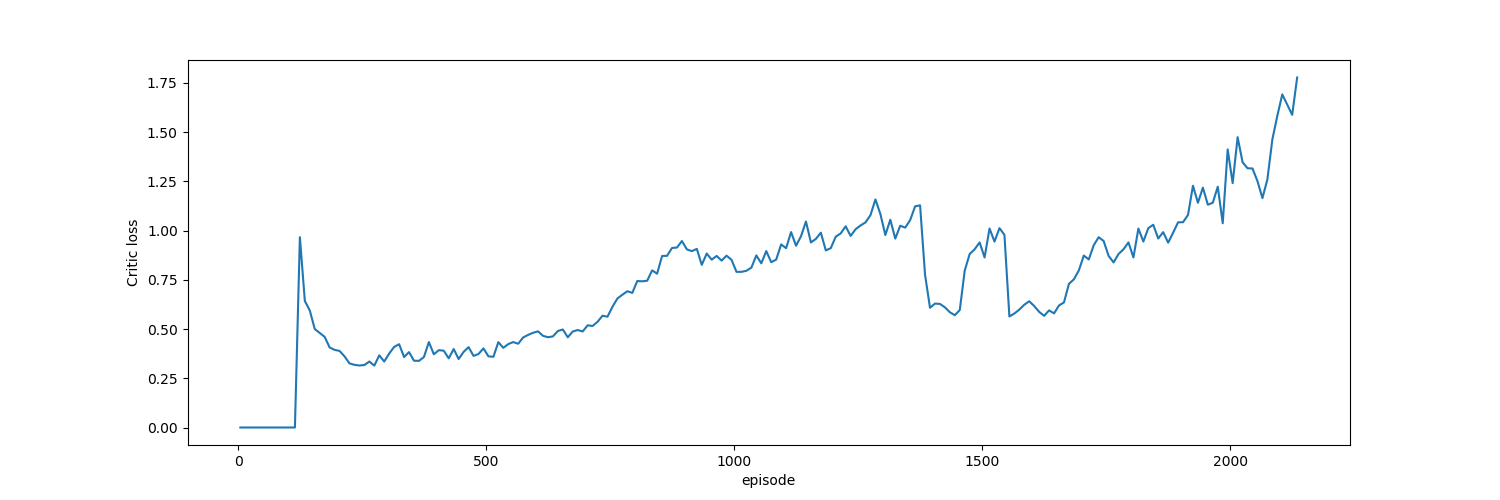
\includegraphics[width=9.5cm, height=4cm]{Critic loss.png}
\caption{Figure 5.3: Critic Loss graph decreases and then fluctuates over time, it suggests that the agent is learning and improving its value function, but may still be exploring different policies or facing some degree of uncertainty in the environment
}\\



\textbf{P max}\\

\graphicspath{ {./images/} }
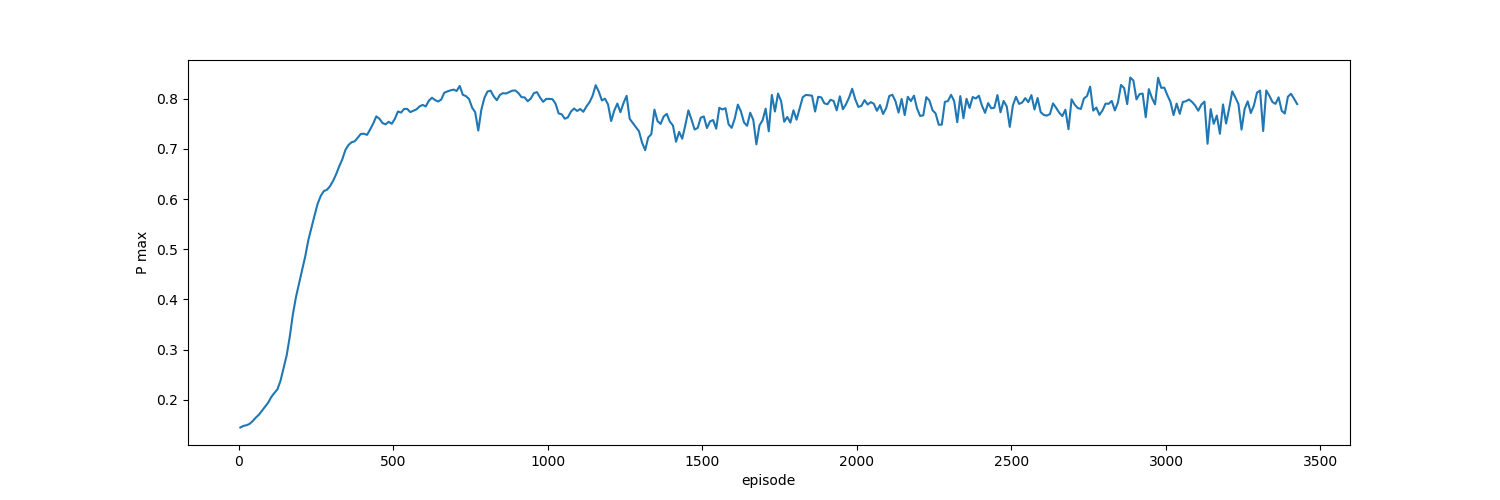
\includegraphics[width=9.5cm, height=4cm]{P max.png}
\caption{Figure 5.4: Pmax graph increases and then plateaus over time, it suggests that the agent is learning to effectively balance exploration and exploitation. The initial increase in the maximum probability of selecting the best action indicates that the agent is improving its policy and becoming more confident in its actions. However, the plateau suggests that the agent has reached a reasonable level of confidence in its policy and is no longer exploring as much, as further exploration may not result in significant improvements in the policy.
 }\\

\textbf{Level}\\

\graphicspath{ {./images/} }
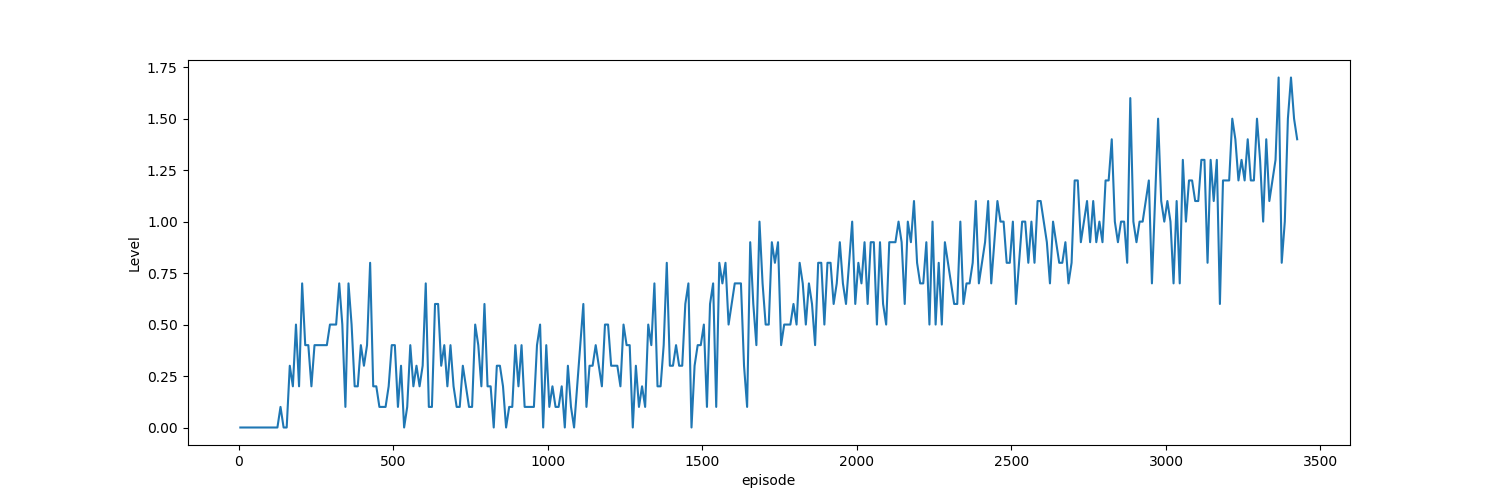
\includegraphics[width=9.5cm, height=4cm]{Level.png}
\caption{Figure 5.5: Level the graph increases over time, it suggests that the agent is improving its performance on the task at hand.
 }\\


\textbf{Score}\\

\graphicspath{ {./images/} }
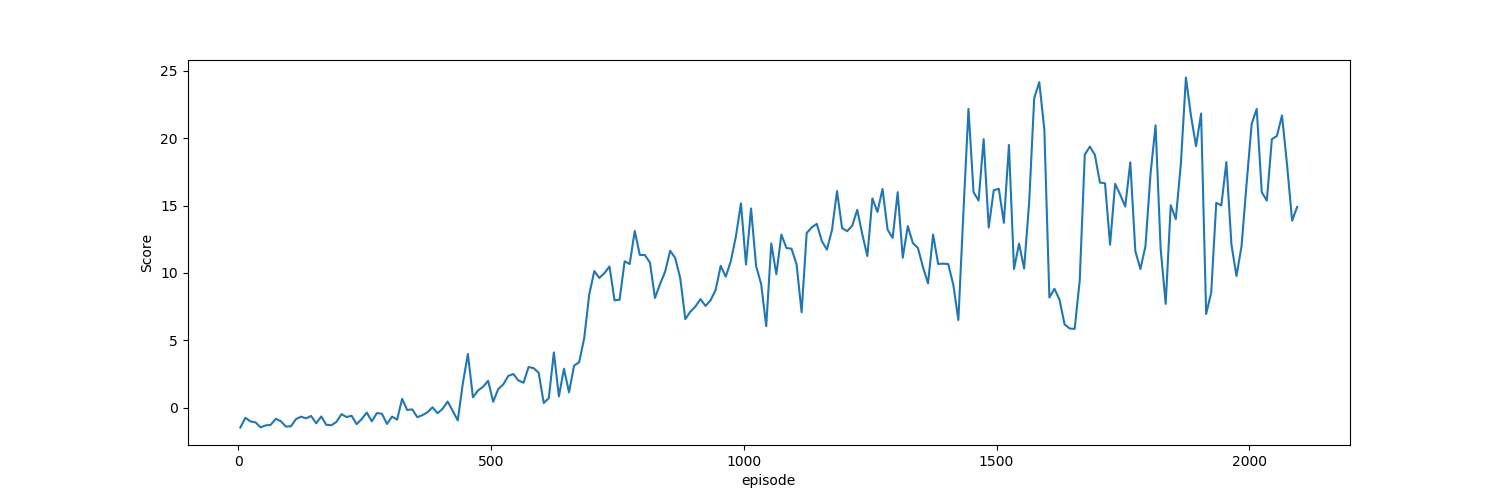
\includegraphics[width=9.5cm, height=4cm]{Score.png}

\caption{Figure 5.6: Score graph increases over time, it suggests that the agent is improving its performance on the task at hand.
}\\

\textbf{Step}\\

\graphicspath{ {./images/} }
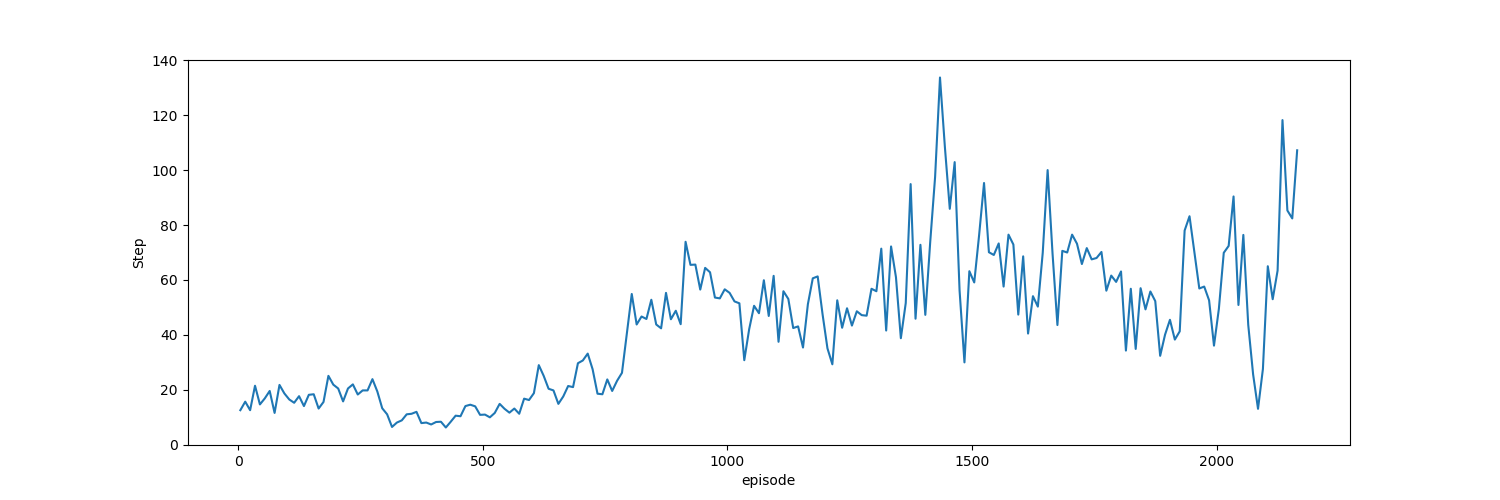
\includegraphics[width=9.5cm, height=4cm]{Step.png}
\caption{Figure 5.7: Step graph increases, decreases, and then increases again over time, it may suggest that the agent is experiencing some level of instability or difficulty in learning the task. This may be because of over-fitting, finding sub-optimal policy or experiencing instability.}\\
 
\\

\subsection{Recurrent Deep Deterministic Policy Gradient}\\

\textbf{RDDPG}\\

The Recurrent Deep Deterministic Policy Gradient (RDPG) algorithm is a type of reinforcement learning algorithm used to train deep neural networks to learn optimal policies for sequential decision-making problems. RDPG is an extension of the Deep Deterministic Policy Gradient (DDPG) algorithm, which itself is a variant of the Q-learning algorithms.\\
It optimizes a policy network and a value network simultaneously. The policy network takes the current state of the environment as input and outputs an action to be taken. The value network takes the current state and the action chosen by the policy network as input and outputs an estimate of the expected return from that state-action pair.\\
It extends DDPG by introducing a recurrent neural network (RNN) into the policy network. The RNN allows the policy network to maintain a memory of past states and actions, which can be used to inform future decisions. This is particularly useful in tasks where the optimal action depends on a sequence of past actions and observations.\\
The policy network is also trained to maximize the expected return over a sequence of actions. The value network is trained to minimize the difference between its estimate of the expected return and the actual return received after taking a sequence of actions. Both networks are updated using backpropagation through time (BPTT), which is a variant of backpropagation that allows gradients to be computed over a sequence of inputs.\\

\textbf{Actor Loss}\\

\graphicspath{ {./images/} }
\includegraphics[width=9.5cm, height=4cm]{Actor loss-2.png}
\caption{Figure 5.8: \textit{Actor loss} graph increases and then decreases over time, it suggests that the agent is exploring different policies and gradually converging to a better solution. The initial increase in the actor loss could be due to the agent trying out different policies and exploring the environment, which may result in suboptimal policies being selected. However, as the agent gains more experience and updates its policy based on the observed rewards, the actor loss should start to decrease again as the agent converges to a better solution.}\\


\textbf{Average Action (Noise)}\\

\graphicspath{ {./images/} }
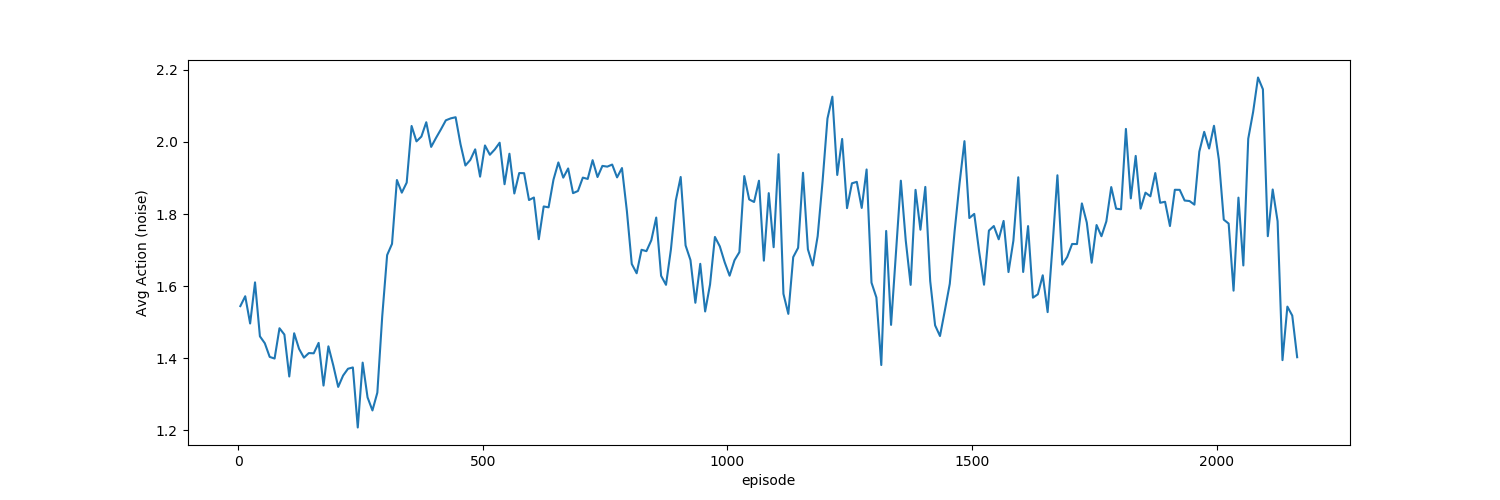
\includegraphics[width=9.5cm, height=4cm]{Avg Action (noise).png}
\caption{Figure 5.9: \textit{Avg Action (noise) }graph fluctuates over time, it suggests that the agent is experiencing some level of instability or variability in its exploration behavior.
}\\

\textbf{Average Q}\\

\graphicspath{ {./images/} }
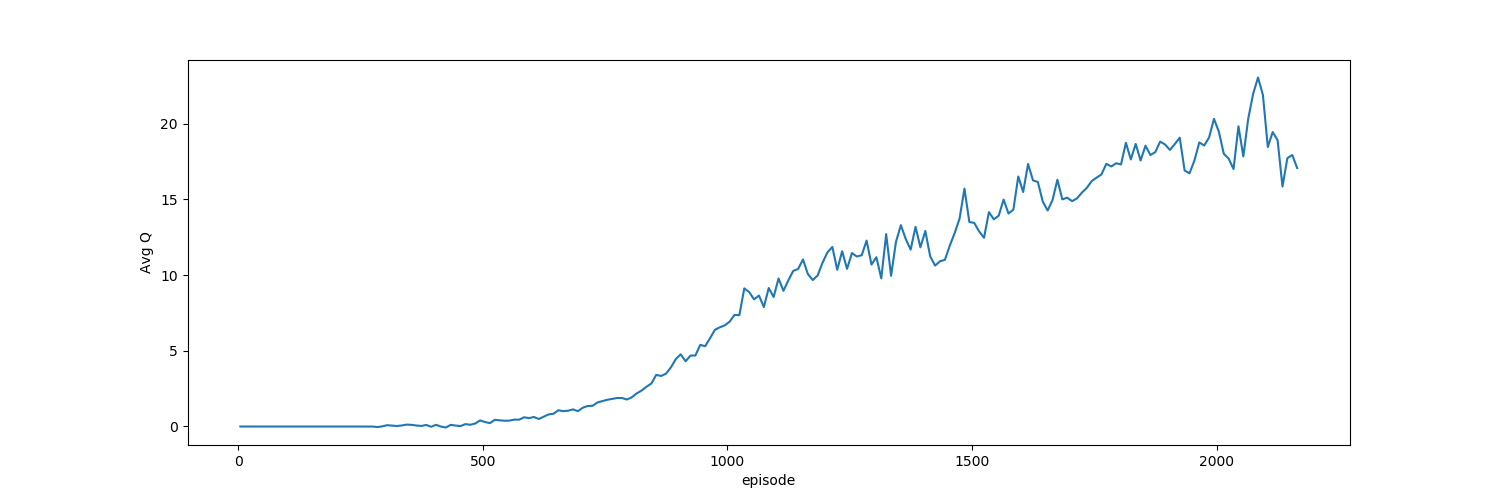
\includegraphics[width=9.5cm, height=4cm]{Avg Q.png}
\caption{Figure 5.10: \textit{Average Q }graph increases over time, it suggests that the agent is improving its estimates of the optimal state-action value function and making better decisions.
}\\


\textbf{Average velocity}\\

\graphicspath{ {./images/} }
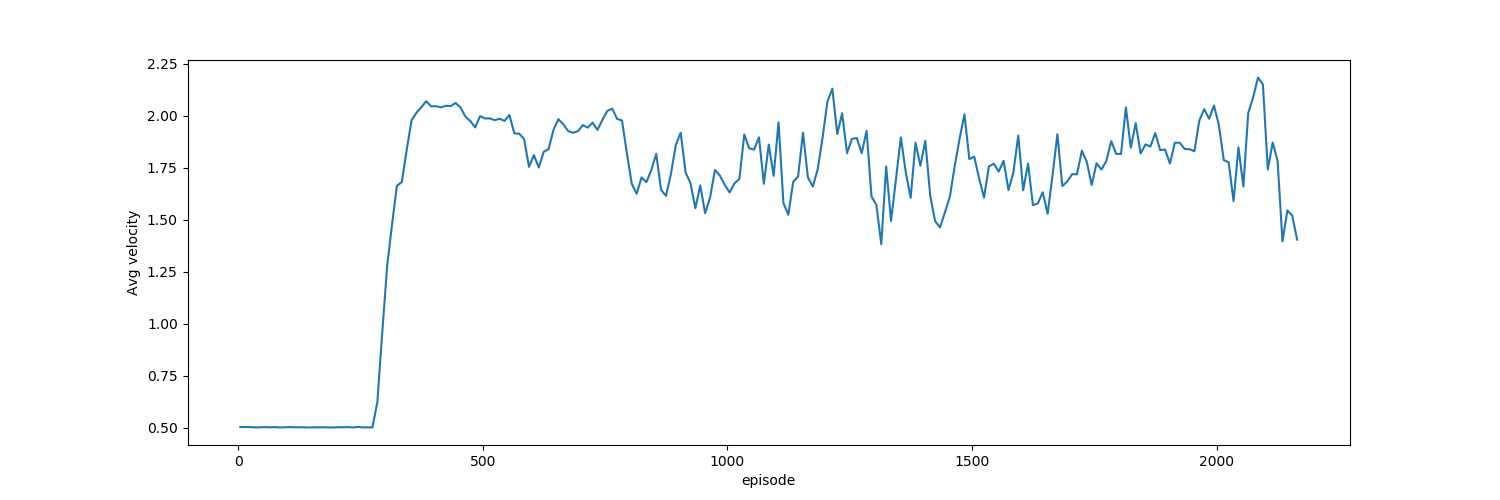
\includegraphics[width=9.5cm, height=4cm]{Avg velocity.png}
\caption{Figure 5.11: \textit{Average velocity }graph increases initially and then plateaus over time, it suggests that the agent is improving its ability to move efficiently through the environment, but has reached a limit in its performance. It may be necessary to adjust the agent's training parameters or explore new techniques to continue improving its performance. Alternatively, it is possible that the plateau in the average velocity is due to the environment itself.
}\\


\textbf{Best Y}\\

\graphicspath{ {./images/} }
\includegraphics[width=9.5cm, height=4cm]{Best Y-2.png}
\caption{Figure 5.12: \textit{Best Y } When this graph increases, it typically means that the agent is learning and improving its performance over time. Specifically, it suggests that the agent is finding better policies for interacting with the environment, resulting in higher rewards or better performance.
}\\


\textbf{Critic Loss}\\

\graphicspath{ {./images/} }
\includegraphics[width=9.5cm, height=4cm]{Critic loss-2.png}
\caption{Figure 5.13: \textit{Critic Loss } graph increases over time, it suggests that the agent is not learning effectively and is not improving its value function as it may have a high learning rate, architecture may not be well suited or the rewards may be delayed.
}\\

\textbf{Level}\\

\graphicspath{ {./images/} }
\includegraphics[width=9.5cm, height=4cm]{Level-2.png}
\caption{Figure 5.14: \textit{Level }graph increases over time, it suggests that the agent is improving its performance on the task at hand.
}\\



\textbf{Score}\\

\graphicspath{ {./images/} }
\includegraphics[width=9.5cm, height=4cm]{Score-2.png}
\caption{Figure 5.15: \textit{Score } graph increases over time, it suggests that the agent is improving its performance on the task at hand
}\\


\textbf{Step}\\

\graphicspath{ {./images/} }
\includegraphics[width=9.5cm, height=4cm]{Step-2.png}
\caption{Figure 5.16: \textit{Step }graph fluctuates over time, it suggests that the agent is experiencing some level of instability in its learning process.
}\\

\subsection{Recurrent Deep Deterministic Policy Gradient}\\

\textbf{RDDPG-PER}\\

The Recurrent Deep Deterministic Policy Gradient (RDPG) algorithm is a type of reinforcement learning algorithm used to train deep neural networks to learn optimal policies for sequential decision-making problems. RDPG is an extension of the Deep Deterministic Policy Gradient (DDPG) algorithm, which itself is a variant of the Q-learning algorithms.\\
It optimizes a policy network and a value network simultaneously. The policy network takes the current state of the environment as input and outputs an action to be taken. The value network takes the current state and the action chosen by the policy network as input and outputs an estimate of the expected return from that state-action pair.\\
It extends DDPG by introducing a recurrent neural network (RNN) into the policy network. The RNN allows the policy network to maintain a memory of past states and actions, which can be used to inform future decisions. This is particularly useful in tasks where the optimal action depends on a sequence of past actions and observations.\\
The policy network is also trained to maximize the expected return over a sequence of actions. The value network is trained to minimize the difference between its estimate of the expected return and the actual return received after taking a sequence of actions. Both networks are updated using backpropagation through time (BPTT), which is a variant of backpropagation that allows gradients to be computed over a sequence of inputs.\\

\textbf{Actor Loss}\\

\graphicspath{ {./images/} }
\includegraphics[width=9.5cm, height=4cm]{Actor loss-3.png}
\caption{Figure 5.17: \textit{Actor loss} graph increases and then decreases over time, it suggests that the agent is exploring different policies and gradually converging to a better solution. The initial increase in the actor loss could be due to the agent trying out different policies and exploring the environment, which may result in suboptimal policies being selected. However, as the agent gains more experience and updates its policy based on the observed rewards, the actor loss should start to decrease again as the agent converges to a better solution.
}\\


\textbf{Average Action (Noise)}\\

\graphicspath{ {./images/} }
\includegraphics[width=9.5cm, height=4cm]{Avg Action (noise)-2.png}
\caption{Figure 5.18: \textit{Avg Action (noise)} graph fluctuates over time, it suggests that the agent is experiencing some level of instability or variability in its exploration behavior.
}\\

\textbf{Average Q}\\

\graphicspath{ {./images/} }
\includegraphics[width=9.5cm, height=4cm]{Avg Q-2.png}
\caption{Figure 5.19: \textit{Average Q }graph increases over time, it suggests that the agent is improving its estimates of the optimal state-action value function and making better decisions.
}\\

\textbf{Average velocity}\\

\graphicspath{ {./images/} }
\includegraphics[width=9.5cm, height=4cm]{Avg velocity-2.png}
\caption{Figure 5.20: \textit{Average velocity} graph increases initially and then plateaus over time, it suggests that the agent is improving its ability to move efficiently through the environment, but has reached a limit in its performance. It may be necessary to adjust the agent's training parameters or explore new techniques to continue improving its performance. Alternatively, it is possible that the plateau in the average velocity is due to the environment itself.
}\\

\textbf{Best Y}\\

\graphicspath{ {./images/} }
\includegraphics[width=9.5cm, height=4cm]{Best Y-3.png}
\caption{Figure 5.21: \textit{Best Y} When this graph increases, it typically means that the agent is learning and improving its performance over time. Specifically, it suggests that the agent is finding better policies for interacting with the environment, resulting in higher rewards or better performance.
}\\

\textbf{Critic Loss}\\

\graphicspath{ {./images/} }
\includegraphics[width=9.5cm, height=4cm]{Critic loss-3.png}
\caption{Figure 5.22: \textit{Critic Loss} graph increases over time, it suggests that the agent is not learning effectively and is not improving its value function as it may have a high learning rate, architecture may not be well suited or the rewards may be delayed.
}\\

\textbf{Level}\\

\graphicspath{ {./images/} }
\includegraphics[width=9.5cm, height=4cm]{Level-3.png}
\caption{Figure 5.23: \textit{Level} graph increases over time, it suggests that the agent is improving its performance on the task at hand
}\\

\textbf{Score}\\

\graphicspath{ {./images/} }
\includegraphics[width=9.5cm, height=4cm]{Score-3.png}
\caption{Figure 5.24: \textit{Score }graph increases over time, it suggests that the agent is improving its performance on the task at hand.
}\\

\textbf{Step}\\

\graphicspath{ {./images/} }
\includegraphics[width=9.5cm, height=4cm]{Step-3.png}
\caption{Figure 5.25 \textit{Step }graph fluctuates over time, it suggests that the agent is experiencing some level of instability in its learning process.
}\\

\subsection{Recurrent Deep Q-Network}\\

\textbf{RDQN}\\

The Recurrent Deep Q-Network (R-DQN) algorithm is an extension of the Deep Q-Network (DQN) algorithm that is designed to work with sequential or time-dependent data.\\
It uses a neural network to approximate the Q-value function, which estimates the expected reward for taking a particular action in a particular state. However, instead of processing each state independently, as in the original DQN, it considers the temporal dependencies between states by using a recurrent neural network (RNN).\\
The RNN allows the algorithm to remember previous states and actions taken, which can be used to inform future decisions. This is especially useful in tasks where the current state is dependent on previous states, such as in video games or robotics.\\
The training process for R-DQN is like DQN, with the algorithm attempting to learn the optimal Q-values by minimizing the difference between the predicted Q-values and the actual Q-values obtained through experience. However, since the RNN introduces additional complexity, the training process is more computationally expensive than DQN.\\

\textbf{Average Q}\\

\graphicspath{ {./images/} }
\includegraphics[width=9.5cm, height=4cm]{Avg Q-3.png}
\caption{Figure 5.26: \textit{Average Q}  graph increases over time, it suggests that the agent is improving its estimates of the optimal state-action value function and making better decisions.
}\\


\textbf{Best Y}\\

\graphicspath{ {./images/} }
\includegraphics[width=9.5cm, height=4cm]{Best Y-4.png}
\caption{Figure 5.27: \textit{Best Y} graph fluctuates for reinforcement algorithms, it means that the performance of the agent is not consistent over time.
}\\

\textbf{Critic Loss}\\

\graphicspath{ {./images/} }
\includegraphics[width=9.5cm, height=4cm]{Critic loss-4.png}
\caption{Figure 5.28: \textit{Critic Loss:} graph increases over time, it suggests that the agent is not learning effectively and is not improving its value function as it may have a high learning rate, architecture may not be well suited or the rewards may be delayed
}\\

\textbf{Level}\\

\graphicspath{ {./images/} }
\includegraphics[width=9.5cm, height=4cm]{Level-4.png}
\caption{Figure 5.29: \textit{Level:} graph increases over time, it suggests that the agent is improving its performance on the task at hand.
}\\

\textbf{Score}\\

\graphicspath{ {./images/} }
\includegraphics[width=9.5cm, height=4cm]{Score-4.png}
\caption{Figure 5.30: \textit{Score: } graph increases over time, it suggests that the agent is improving its performance on the task at hand
}\\

\textbf{Step}\\

\graphicspath{ {./images/} }
\includegraphics[width=9.5cm, height=4cm]{Step-4.png}
\caption{Figure 5.31: \textit{Step: }graph fluctuates over time, it suggests that the agent is experiencing some level of instability in its learning process.
}\\

\subsection{Twin Delayed Deep Deterministic Policy Gradient}\\

\textbf{TD3-PER}\\

TD3 (Twin Delayed Deep Deterministic Policy Gradient) is a reinforcement learning algorithm that can be used for continuous control tasks. PER (Prioritized Experience Replay) is an extension of the standard experience replay technique that prioritizes the replay of certain experiences based on their estimated importance.\\
In this, two Q-networks are used to estimate the value function of state-action pairs. The policy is updated by minimizing the loss function between the Q-value and the target value, which is calculated as the sum of the reward and the discounted Q-value of the next state as estimated by the target network. To prevent overestimation of the Q-values, a target network is used that is updated less frequently than the main network. \\Additionally, noise is added to the action selection process to encourage exploration.\\
To incorporate PER into TD3, the priority of each experience is used to weight the loss function during the policy update. Specifically, the loss function is multiplied by a weight factor that is proportional to the priority of the experience. Additionally, the replay buffer is updated using a stochastic prioritization method, which allows for a balance between prioritization and random sampling. Overall, the combination of TD3 and PER can lead to improved learning and faster convergence in continuous control tasks.\\

\textbf{Actor Loss}\\

\graphicspath{ {./images/} }
\includegraphics[width=9.5cm, height=4cm]{Actor loss-4.png}
\caption{Figure 5.32: \textit{Actor loss}: graph increases over time, it suggests that the agent is not learning effectively and is not improving its policy. This may be because the learning rate may be too high, the architecture is not suitable , or the reward may be delayed.
}\\

\textbf{Average Action (Noise)}\\

\graphicspath{ {./images/} }
\includegraphics[width=9.5cm, height=4cm]{Avg Action (noise)-3.png}
\caption{Figure 5.33: \textit{Avg Action (noise) } graph fluctuates over time, it suggests that the agent is experiencing some level of instability or variability in its exploration behavior.
}\\

\textbf{Average Q}\\

\graphicspath{ {./images/} }
\includegraphics[width=9.5cm, height=4cm]{Avg Q-4.png}
\caption{Figure 5.34: \textit{Average Q :}  graph increases over time, it suggests that the agent is improving its estimates of the optimal state-action value function and making better decisions.
}\\


\textbf{Average velocity}\\

\graphicspath{ {./images/} }
\includegraphics[width=9.5cm, height=4cm]{Avg velocity-3.png}
\caption{Figure 5.35: \textit{Average velocity: } graph increases initially and then plateaus over time, it suggests that the agent is improving its ability to move efficiently through the environment, but has reached a limit in its performance. It may be necessary to adjust the agent's training parameters or explore new techniques to continue improving its performance. Alternatively, it is possible that the plateau in the average velocity is due to the environment itself.
}\\

\textbf{Best Y}\\

\graphicspath{ {./images/} }
\includegraphics[width=9.5cm, height=4cm]{Best Y-5.png}
\caption{Figure 5.36: \textit{Best Y: } When this graph increases, it typically means that the agent is learning and improving its performance over time. Specifically, it suggests that the agent is finding better policies for interacting with the environment, resulting in higher rewards or better performance.
}\\

\textbf{Critic Loss}\\

\graphicspath{ {./images/} }
\includegraphics[width=9.5cm, height=4cm]{Critic loss-5.png}
\caption{Figure 5.37: \textit{Critic Loss:}  graph increases over time, it suggests that the agent is not learning effectively and is not improving its value function as it may have a high learning rate, architecture may not be well suited or the rewards may be delayed.
}\\

\textbf{Level}\\

\graphicspath{ {./images/} }
\includegraphics[width=9.5cm, height=4cm]{Level-5.png}
\caption{Figure 5.38: \textit{Level:} graph increases over time, it suggests that the agent is improving its performance on the task at hand.
}\\

\textbf{Score}\\

\graphicspath{ {./images/} }
\includegraphics[width=9.5cm, height=4cm]{Score-5.png}
\caption{Figure 5.39: \textit{Score }graph increases over time, it suggests that the agent is improving its performance on the task at hand.
}\\

\textbf{Step}\\

\graphicspath{ {./images/} }
\includegraphics[width=9.5cm, height=4cm]{Step-5.png}
\caption{Figure 5.40:\textit{Step: }graph increases over time, it suggests that the agent is improving its performance on the task at hand.
}\\

\subsection{Proximal Policy Optimization}\\

\textbf{PPO}\\

PPO (Proximal Policy Optimization) is a reinforcement learning algorithm used for training agent-based systems that can learn to perform tasks in an environment. It is an improvement over the classic policy gradient algorithm, which suffers from high variance and instability issues. It uses an objective function that includes two terms: a clipped surrogate objective and an entropy bonus. The clipped surrogate objective is used to constrain the size of policy updates so that the changes are not too large, which helps to prevent the agent from diverging too far from its current policy. The entropy bonus encourages exploration and prevents the agent from becoming too certain about its actions.\\
The PPO algorithm operates in two phases: sampling and optimization. During the sampling phase, the agent collects a set of trajectories by taking actions in the environment. These trajectories are used to estimate the expected returns and advantages for each state-action pair. The advantages represent how much better or worse the agent's actions were compared to a baseline, which is typically the value function estimated by a critic.\\
In the optimization phase, the clipped surrogate objective is maximized using a batch of collected trajectories. The clipping mechanism ensures that the policy updates are not too large, which helps to stabilize the training process. The entropy bonus is also added to the objective to encourage exploration.\\


\textbf{Best Y}\\

\graphicspath{ {./images/} }
\includegraphics[width=9.5cm, height=4cm]{Best Y-6.png}
\caption{Figure 5.41: \textit{Best Y: }When this graph increases, it typically means that the agent is learning and improving its performance over time. Specifically, it suggests that the agent is finding better policies for interacting with the environment, resulting in higher rewards or better performance.
}\\



\textbf{\textit{Comparison Results for the algorithms based on various parameters : }}
\begin{enumerate}
    \item Best Record\\
    \graphicspath{ {./images/} }
    \includegraphics[width=9cm, height=4cm]{result_Best Record 2.png}
    \caption{Figure 5.42: The X axis denotes the number of episodes and the Y axis denotes the Best Record parameter.\\
    }\\

    \item Getting Goal Probability\\
    \graphicspath{ {./images/} }
    \includegraphics[width=9cm, height=4cm]{result_Get Goal Prob. 2.png}
    \caption{Figure 5.43: The X axis denotes the number of episodes and the Y axis denotes the getting goal probability parameter.\\
    }\\

    \item Step for Goal\\
    \graphicspath{ {./images/} }
    \includegraphics[width=8.5cm, height=4cm]{result_Step for Goal 2.png}
    \caption{Figure 5.44: The X axis denotes the number of episodes and the Y axis denotes the step for goal parameter.\\
    }\\

    \item Step per Record\\
    \graphicspath{ {./images/} }
    \includegraphics[width=8.5cm, height=4cm]{result_Step per Record 2.png}
    \caption{Figure 5.45: The X axis denotes the number of episodes and the Y axis denotes the step per record parameter.\\
    }\\

    \item Step \\
    \graphicspath{ {./images/} }
    \includegraphics[width=8.5cm, height=4cm]{result_Step 2.png}}
    \caption{Figure 5.46: The X axis denotes the number of episodes and the Y axis denotes the step parameter.\\
    }\\

    \item Power Comparison\\
    \graphicspath{ {./images/} }
    \includegraphics[width=6.5cm, height=4cm]{energy_power_density.png}}\\
    \caption{Figure 5.47: The power density vs. the energy density relative to present-day technology. \\
    }\\
    

    
\end{enumerate}

\section{Conclusion}

In conclusion, DecentraliDrone is an innovative drone delivery system that has the potential to revolutionize the way we transport goods. By leveraging advanced technology and a decentralized architecture, DecentraliDrone is able to operate autonomously and efficiently, without the need for human intervention. The system has numerous potential applications, from delivering medical supplies to remote areas to transporting goods between urban centers.

While there are still challenges that need to be addressed, such as developing robust communication protocols and ensuring the safety and security of the system, the progress that has been made so far is promising. The successful simulation of the system using the TD3-PER algorithm provides a strong foundation for future work, which will involve application development, hardware deployment, and field testing.

Overall, DecentraliDrone represents a promising step forward in the field of autonomous delivery systems, and has the potential to bring us closer to a more interconnected and efficient world.




\begin{thebibliography}{1}

\bibitem{li2018review}
J.~Li, M.~Zhou, and N.~Wang, ``A review of key technologies and applications of decentralized autonomous drone delivery systems,'' \emph{IEEE Transactions on Industrial Informatics}, vol.~14, no.~8, pp. 3588--3597, 2018.

\bibitem{zhou2018routing}
M.~Zhou, J.~Li, and N.~Wang, ``Routing algorithms and communication protocols for decentralized autonomous drone delivery systems: A review,'' \emph{IEEE Access}, vol.~6, pp. 50,762--50,776, 2018.

\bibitem{wang2018survey}
N.~Wang, M.~Zhou, and J.~Li, ``A survey of decentralized autonomous drone delivery systems: Design approaches, applications, and challenges,'' \emph{IEEE Transactions on Industrial Informatics}, vol.~14, no.~8, pp. 3598--3607, 2018.

\bibitem{kegeleirs2021swarm}
M. ~Kegeleirs, G. ~Grisetti, and M. ~Birattari, “Swarm SLAM: Challenges and Perspectives,” \emph{Frontiers} in Robotics and AI, vol. ~8, Mar. 2021, doi: 10.3389/frobt.2021.618268.

\bibitem{chen2022end}
S. ~Chen, W. ~Zhou, A.-S. ~Yang, H. ~Chen, B. ~Li, and C.-Y. ~Wen, “An End-to-End UAV Simulation Platform for Visual SLAM and Navigation,” \emph{Aerospace}, vol. ~9, no. ~2, p. 48, Jan. 2022, doi: 10.3390/aerospace9020048.

\bibitem{gupta2022slam}
A. ~Gupta and X. ~Fernando, “Simultaneous Localization and Mapping (SLAM) and Data Fusion in Unmanned Aerial Vehicles: Recent Advances and Challenges,” \emph{Drones}, vol. ~6, no. ~4, p. 85, Mar. 2022, doi: 10.3390/drones6040085.

\bibitem{munguía2016vslam}
R. ~Munguía, S. Urzua, Y. Bolea, and A. Grau, “Vision-Based SLAM System for Unmanned Aerial Vehicles,” \emph{Sensors}, vol. ~16, no. ~3, p. 372, Mar. 2016, doi: 10.3390/s16030372.

\bibitem{lópez2017sensorial}
E. ~López et al., “A Multi-Sensorial Simultaneous Localization and Mapping (SLAM) System for Low-Cost Micro Aerial Vehicles in GPS-Denied Environments,” \emph{Sensors}, vol. 17, no. 4, p. 802, Apr. 2017, doi: 10.3390/s17040802.

\bibitem{mahdoui2019multiUAV}
N. ~Mahdoui, V. ~Frémont, and E. ~Natalizio, “Communicating Multi-UAV System for Cooperative SLAM-based Exploration,” Journal of Intelligent &amp; \emph{Robotic Systems}, vol. 98, no. 2, pp. 325–343, Nov. 2019, doi: 10.1007/s10846-019-01062-6.

\bibitem{xu2022decentalized}
H. ~Xu, P. ~Liu, X. ~Chen, S. ~Shen, “Decentralized and distributed collaborative simultaneous localization and mapping system for aerial swarms”, doi: 10.14711/thesis-991013142455303412.

\bibitem{jarrah2022flight}
K. ~Jarrah, Y. ~Alali, A. ~Lalko, and O. ~Rawashdeh, “Flight Time Optimization and Modeling of a Hybrid Gasoline–Electric Multirotor Drone: An Experimental Study,” \emph{Aerospace}, vol. 9, no. 12, p. 799, Dec. 2022, doi: 10.3390/aerospace9120799.

\bibitem{stolaroff2018energy}
J. K. ~Stolaroff, C. ~Samaras, E. R. ~O’Neill, A. ~Lubers, A. S. ~Mitchell, and D. ~Ceperley, “Energy use and life cycle greenhouse gas emissions of drones for commercial package delivery,” \emph{Nature Communications}, vol. 9, no. 1, Feb. 2018, doi: 10.1038/s41467-017-02411-5.

\bibitem{arshad2021loop}
S. ~Arshad and G.-W. ~Kim, “Role of Deep Learning in Loop Closure Detection for Visual and Lidar SLAM: A Survey,” \emph{Sensors}, vol. 21, no. 4, p. 1243, Feb. 2021, doi: 10.3390/s21041243.

\bibitem{chen2022coverage}
J. ~Chen, C. ~Du, Y. ~Zhang, P. ~Han, and W. ~Wei, “A Clustering-Based Coverage Path Planning Method for Autonomous Heterogeneous UAVs,” \emph{IEEE Transactions on Intelligent Transportation Systems}, vol. 23, no. 12, pp. 25546–25556, Dec. 2022, doi: 10.1109/tits.2021.3066240.

\bibitem{yang2021rrt}
S. M. ~Yang and Y. A. ~Lin, “Development of an Improved Rapidly Exploring Random Trees Algorithm for Static Obstacle Avoidance in Autonomous Vehicles,” \emph{Sensors}, vol. 21, no. 6, p. 2244, Mar. 2021, doi: 10.3390/s21062244.

\bibitem{debeunne2020vlidar}
C. ~Debeunne and D. ~Vivet, “A Review of Visual-LiDAR Fusion based Simultaneous Localization and Mapping,” \emph{Sensors}, vol. 20, no. 7, p. 2068, Apr. 2020, doi: 10.3390/s20072068.

\bibitem{karur2021path}
K. ~Karur, N. ~Sharma, C. ~Dharmatti, and J. E. ~Siegel, “A Survey of Path Planning Algorithms for Mobile Robots,” \emph{Vehicles}, vol. 3, no. 3, pp. 448–468, Aug. 2021, doi: 10.3390/vehicles3030027.

\bibitem{cui2017brief}
Q. ~Cui, P. ~Liu, J. ~Wang, and J. ~Yu, “Brief analysis of drone swarms communication,” 2017 \emph{IEEE International Conference on Unmanned Systems (ICUS)}, Oct. 2017, doi: 10.1109/icus.2017.8278390.

\bibitem{innocente2019self}
M. S. ~Innocente and P. ~Grasso, “Self-organising swarms of firefighting drones: Harnessing the power of collective intelligence in decentralised multi-robot systems,” \emph{Journal of Computational Science}, vol. ~34, pp. 80–101, May 2019, doi: 10.1016/j.jocs.2019.04.009.

\bibitem{kyriakakis2021moving}
N. A. Kyriakakis, M. Marinaki, N. Matsatsinis, and Y. Marinakis, “Moving peak drone search problem: An online multi-swarm intelligence approach for UAV search operations,” Swarm and Evolutionary Computation, vol. 66, p. 100956, Oct. 2021, doi: 10.1016/j.swevo.2021.100956.

\bibitem{bartolini2020druber}
N. Bartolini, A. Coletta, G. Maselli, and M. Piva, “DRUBER,” Proceedings of the 6th ACM Workshop on Micro Aerial Vehicle Networks, Systems, and Applications, Jun. 2020, doi: 10.1145/3396864.3399706.

\bibitem{chen2010hybrid}
H. ~Chen and A. ~Khaligh, “Hybrid energy storage system for unmanned aerial vehicle (UAV),” \emph{IECON 2010 - 36th Annual Conference on IEEE Industrial Electronics Society}, Nov. 2010, doi: 10.1109/iecon.2010.5675076.

\bibitem{islam2019path}
S. ~Islam and A. ~Razi, “A Path Planning Algorithm for Collective Monitoring Using Autonomous Drones,” 2019 53rd \emph{Annual Conference on Information Sciences and Systems (CISS)}, Mar. 2019, doi: 10.1109/ciss.2019.8693023.

\bibitem{hong2021energy}
D. ~Hong, S. ~Lee, Y. H. ~Cho, D. ~Baek, J. ~Kim, and N. ~Chang, “Energy-Efficient Online Path Planning of Multiple Drones Using Reinforcement Learning,” \emph{IEEE Transactions on Vehicular Technology}, vol. 70, no. 10, pp. 9725–9740, Oct. 2021, doi: 10.1109/tvt.2021.3102589.

\bibitem{xu2022omni}
H. ~Xu et al., “Omni-Swarm: A Decentralized Omnidirectional Visual–Inertial–UWB State Estimation System for Aerial Swarms,” \emph{IEEE Transactions on Robotics}, vol. 38, no. 6, pp. 3374–3394, Dec. 2022, doi: 10.1109/tro.2022.3182503.


\end{thebibliography}

\end{document}